\documentclass{article}
\pagenumbering{arabic}
\usepackage{graphicx,amsmath,amssymb,bm,tikz}
\usetikzlibrary{calc,patterns,decorations.pathmorphing,decorations.markings}
\usepackage{xfrac}
\usepackage[utf8]{inputenc}
\usepackage{hyperref}
% Format fref 
\usepackage[plain,english]{fancyref}
\usepackage[margin=1in]{geometry} 
\fancyrefaddcaptions{english}{\renewcommand*{\frefeqname}{Eq.}}
% Figure Packages
\usepackage[outercaption]{sidecap}
\usepackage[export]{adjustbox}
\usepackage{graphicx}
\usepackage{caption}
\usepackage{wrapfig}
\usepackage{float}
\usepackage{algorithm, algorithmic, amsfonts,amsmath,amssymb,amsthm, color,comment,enumitem, environ, fancyhdr,   graphicx, mathtools, wasysym}
\pagestyle{fancy}
\setlength{\headheight}{22.5pt}
\newenvironment{problem}[2][Problem]{\begin{trivlist}
\item[\hskip \labelsep {\bfseries #1}\hskip \labelsep {\bfseries #2.}]}{\end{trivlist}}
\newenvironment{sol}
    {\emph{Solution:}
    }
    {
    \qed
    }
\specialcomment{com}{ \color{blue} \textbf{Comment:} }{\color{black}} %for instructor comments while grading
\NewEnviron{probscore}{\marginpar{ \color{blue} \tiny Problem Score: \BODY \color{black} }}
%%%%%%%%%%%%%%%%%%%%%%%%%%%%%%%%%%%%%%%%%%%%%%%%%%%%%%%%%%%%%%%%%%%%%%%%%%%%%%%%%





%%%%%%%%%%%%%%%%%%%%%%%%%%%%%%%%%%%%%%%%%%%%%
%Fill in the appropriate information below
\lhead{Daniel Agramonte}  %replace with your name
\rhead{MCHE 6390 \\ Project 1 - Final Report} %replace XYZ with the homework course number, semester (e.g. ``Spring 2019"), and assignment number.
%%%%%%%%%%%%%%%%%%%%%%%%%%%%%%%%%%%%%%%%%%%%%



% Table stuff
\usepackage{multirow}
%\usepackage{floatrow}
%	\floatsetup[table]{capposition=top}%puts table caption above
% Change \subsection title characteristics
    \usepackage[parfill]{parskip}   % forces parskip to not affect headings
    \usepackage{enumitem}           % used for editing itemize environment
    \usepackage{titlesec}
        \titleformat*{\section}{\Large\bfseries\titlerule\vspace{0.5em}}
% Quote blocks
    \usepackage{csquotes} % use environment 'displayquote'
% Misc document settings
    \title{\Huge MCHE 6390 Project 1 - Prelab Work} \author{Daniel Agramonte} \date{10.30.20}
    \setlength{\parindent}{0pt}
    \setlength{\parskip}{1em}
    \setlist{nosep, itemsep=0pt, parsep=0pt}
% Misc vocab commands
    \newcommand{\msalg}{{\fontfamily{cmtt}\selectfont ms83}}
    \newcommand{\lsq}{\emph{lsqnonlin}}
    \newcommand{\msalge}{{\fontfamily{cmtt}\selectfont MCHE\_6500\_NIST\_POLY}}
%
% MATLAB packages
%
\usepackage[framed,numbered]{matlab-prettifier}
\usepackage{textcomp}
\usepackage{listings}
%
% Matrix Spacing
%
\makeatletter
\renewcommand*\env@matrix[1][\arraystretch]{%
  \edef\arraystretch{#1}%
  \hskip -\arraycolsep
  \let\@ifnextchar\new@ifnextchar
  \array{*\c@MaxMatrixCols c}}
\makeatother
%
\begin{document}
\maketitle
\section*{Executive Summary}
In this report, we create a theoretical 3 degree of freedom lumped sum model for a 3 story building and validated it theoretically using Experimental Modal Analysis (EMA). We found that the by varying the effective stiffness of the springs that we could achieve a maximum absolute error of only 6.93\%. The modes had the correct shape, but the minimum error we achieved was significantly higher at 40.53\%.   
\section*{Modeling}
We first present our first order, two dimensional model of the following system. We assume that each floor will only move laterally in plane, and that each floor is connected with bars in perfect fixed-fixed boundary conditions.

From this, we can then develop a lumped parameter model as follows.
\\ \\
\begin{tikzpicture}
\tikzstyle{spring}=[thick,decorate,decoration={zigzag,pre length=0.3cm,post length=0.3cm,segment length=6}]
\tikzstyle{damper}=[thick,decoration={markings,  
  mark connection node=dmp,
  mark=at position 0.5 with 
  {
    \node (dmp) [thick,inner sep=0pt,transform shape,rotate=-90,minimum width=15pt,minimum height=3pt,draw=none] {};
    \draw [thick] ($(dmp.north east)+(2pt,0)$) -- (dmp.south east) -- (dmp.south west) -- ($(dmp.north west)+(2pt,0)$);
    \draw [thick] ($(dmp.north)+(0,-5pt)$) -- ($(dmp.north)+(0,5pt)$);
  }
}, decorate]
\tikzstyle{ground}=[fill,pattern=north east lines,draw=none,minimum width=0.75cm,minimum height=0.3cm]
% Mass 1
\begin{scope}[xshift=7cm]
\node (M) [minimum width=2.5cm, minimum height=2.5cm] {$m_{1}$};
\draw (-1.25,-1.25) rectangle (1.25,1.25);
\node (ground) [ground,anchor=north,yshift=-0.25cm,minimum width=3.cm] at (M.south) {};
\draw (ground.north east) -- (ground.north west);
\draw [thick] (M.south west) ++ (0.25cm,-0.125cm) circle (0.125cm)  (M.south east) ++ (-0.25cm,-0.125cm) circle (0.125cm);
\node (wall) [ground, rotate=-90, minimum width=3cm,yshift=-3cm] {};
\draw (wall.north east) -- (wall.north west);
% Spring + spring constant
\draw [spring] ($(wall.east)+(0.15,2cm)$) -- ($(M.west)+(0,0.5cm)$);
\node [above right] at (-2.25,-0.05) {$k_1$};
% Damper + coefficient of linear viscous damping
\draw [damper] ($(wall.east)+(0.15,1cm)$) -- ($(M.west)+(0,-0.5cm)$);
\node [above right] at (-2.25,-1.25) {$c_1$};
% Coordinate System
\draw [thick,gray,->] (0,1.5) -- (0.5,1.5) node[right] {$+x_{1}$};
\draw [thick,gray,-] (0,1.25) -- (0,1.5);
\end{scope}
% Mass 2
\begin{scope}[xshift=11cm]
\node (M) [minimum width=2.5cm, minimum height=2.5cm] {$m_{2}$};
\draw (-1.25,-1.25) rectangle (1.25,1.25);
\node (ground) [ground,anchor=north,yshift=-0.25cm,minimum width=3.cm] at (M.south) {};
\draw (ground.north east) -- (ground.north west);
\draw [thick] (M.south west) ++ (0.25cm,-0.125cm) circle (0.125cm)  (M.south east) ++ (-0.25cm,-0.125cm) circle (0.125cm);
% Spring + Spring Constant
\draw [spring] ($(wall.east)+(4.25,2cm)$) -- ($(M.west)+(0,0.5cm)$);
\node [above right] at (-2.25,-0.05) {$k_2$};
% Damper + coefficient of linear viscous damping
\draw [damper] ($(wall.east)+(4.25,1cm)$) -- ($(M.west)+(0,-0.5cm)$);
\node [above right] at (-2.25,-1.25) {$c_2$};
% Coordinate System
\draw [thick,gray,->] (0,1.5) -- (0.5,1.5) node[right] {$+x_{2}$};
\draw [thick,gray,-] (0,1.25) -- (0,1.5);
\end{scope}
% Mass 3
\begin{scope}[xshift=15cm]
\node (M) [minimum width=2.5cm, minimum height=2.5cm] {$m_{3}$};
\draw (-1.25,-1.25) rectangle (1.25,1.25);
\node (ground) [ground,anchor=north,yshift=-0.25cm,minimum width=3.cm] at (M.south) {};
\draw (ground.north east) -- (ground.north west);
\draw [thick] (M.south west) ++ (0.25cm,-0.125cm) circle (0.125cm)  (M.south east) ++ (-0.25cm,-0.125cm) circle (0.125cm);
% Spring + Spring Constant
\draw [spring] ($(wall.east)+(8.25,2cm)$) -- ($(M.west)+(0,0.5cm)$);
\node [above right] at (-2.25,-0.05) {$k_3$};
% Damper + Coefficient of linear viscous damping
\draw [damper] ($(wall.east)+(8.25,1cm)$) -- ($(M.west)+(0,-0.5cm)$);
\node [above right] at (-2.25,-1.25) {$c_3$};
% Coordinate System
\draw [thick,gray,->] (0,1.5) -- (0.5,1.5) node[right] {$+x_{3}$};
\draw [thick,gray,-] (0,1.25) -- (0,1.5);
\end{scope}
\end{tikzpicture} \hfill \break
\noindent With this lumped parameter model, we can develop equations to describe the system using Newton's Second Law.

Assembling these equations,
\begin{flalign*}
    m_{1}\ddot{x}_{1}&+(c_{1}+c_{2})\dot{x}_{1}-c_{2}\dot{x}_{2}+(k_{1}+k_{2})x_{1}-k_{2}x_{2} = 0&& \\
    m_{2}\ddot{x}_{2}&-c_{2}\dot{x}_{1}+(c_{2}+c_{3})\dot{x}_{2}-c_{3}\dot{x}_{3}-k_{2}x_{1}+(k_{2}+k_{3})x_{2}-k_{3}x_{3} = 0&& \\
    m_{3}\ddot{x}_{3}&-c_{3}\dot{x}_{2}+c_{3}\dot{x}_{3}-k_{3}x_{2}+k_{3}x_{3} = 0&& \\
    \begin{bmatrix}
    m_{1} & 0     & 0     \\
    0     & m_{2} & 0     \\
    0     & 0     & m_{3}
    \end{bmatrix}
    &
    \begin{bmatrix}
    \ddot{x}_{1}    \\
    \ddot{x}_{2}    \\
    \ddot{x}_{3}     
    \end{bmatrix}
    +
    \begin{bmatrix}
    c_{1}+c_{2} & -c_{2}      & 0      \\
    -c_{2}      & c_{2}+c_{3} & -c_{3} \\
    0           & -c_{3}      & c_{3}
    \end{bmatrix}
    \begin{bmatrix}
    \dot{x}_{1}    \\
    \dot{x}_{2}    \\
    \dot{x}_{3}     
    \end{bmatrix}
    +
    \begin{bmatrix}
    k_{1}+k_{2} & -k_{2}      & 0      \\
    -k_{2}      & k_{2}+k_{3} & -k_{3} \\
    0           & -k_{3}      & k_{3}
    \end{bmatrix}
    \begin{bmatrix}
    x_{1}    \\
    x_{2}    \\
    x_{3}     
    \end{bmatrix}
    =
    \begin{bmatrix}
    0    \\
    0    \\
    0     
    \end{bmatrix}.
\end{flalign*}
Now we apply the modal coordinate transformation and rewrite the equations as
\begin{flalign*}
    U^{T}
    \begin{bmatrix}
    m_{1} & 0     & 0     \\
    0     & m_{2} & 0     \\
    0     & 0     & m_{3}
    \end{bmatrix}
    &
    U
    \begin{bmatrix}
    \ddot{r}_{1}    \\
    \ddot{r}_{2}    \\
    \ddot{r}_{3}     
    \end{bmatrix}
    +
    U^{T}
    \begin{bmatrix}
    c_{1}+c_{2} & -c_{2}      & 0      \\
    -c_{2}      & c_{2}+c_{3} & -c_{3} \\
    0           & -c_{3}      & c_{3}
    \end{bmatrix}
    U
    \begin{bmatrix}
    \dot{r}_{1}    \\
    \dot{r}_{2}    \\
    \dot{r}_{3}     
    \end{bmatrix}
    +
    U^{T}
    \begin{bmatrix}
    k_{1}+k_{2} & -k_{2}      & 0      \\
    -k_{2}      & k_{2}+k_{3} & -k_{3} \\
    0           & -k_{3}      & k_{3}
    \end{bmatrix}
    U
    \begin{bmatrix}
    r_{1}    \\
    r_{2}    \\
    r_{3}     
    \end{bmatrix}
    =
    \begin{bmatrix}
    0    \\
    0    \\
    0     
    \end{bmatrix}
    && \\
    \begin{bmatrix}
    1 & 0 & 0     \\
    0 & 1 & 0     \\
    0 & 0 & 1
    \end{bmatrix}&
    \begin{bmatrix}
    \ddot{r}_{1}    \\
    \ddot{r}_{2}    \\
    \ddot{r}_{3}     
    \end{bmatrix}
    +
    U^{T}
    \begin{bmatrix}
    c_{1}+c_{2} & -c_{2}      & 0      \\
    -c_{2}      & c_{2}+c_{3} & -c_{3} \\
    0           & -c_{3}      & c_{3}
    \end{bmatrix}
    U
    \begin{bmatrix}
    \dot{r}_{1}    \\
    \dot{r}_{2}    \\
    \dot{r}_{3}     
    \end{bmatrix}
    +
    \begin{bmatrix}
    \omega_{n_{1}}^{2} & 0                  & 0     \\
    0                  & \omega_{n_{2}}^{2} & 0     \\
    0                  & 0                  & \omega_{n_{3}}^{2}
    \end{bmatrix}
    \begin{bmatrix}
    r_{1}    \\
    r_{2}    \\
    r_{3}     
    \end{bmatrix}
    =
    \begin{bmatrix}
    0    \\
    0    \\
    0     
    \end{bmatrix}.&&
\end{flalign*}
Applying the approximation that 
\begin{flalign*}
    U^{T}
    \begin{bmatrix}
    c_{1}+c_{2} & -c_{2}      & 0      \\
    -c_{2}      & c_{2}+c_{3} & -c_{3} \\
    0           & -c_{3}      & c_{3}
    \end{bmatrix}
    U
    \begin{bmatrix}
    \dot{r}_{1}    \\
    \dot{r}_{2}    \\
    \dot{r}_{3}     
    \end{bmatrix}
    =
    \begin{bmatrix}
    2\zeta_{1}\omega_{n_{1}} & 0 & 0      \\
    0 & 2\zeta_{2}\omega_{n_{2}} & 0 \\
    0 & 0 & 2\zeta_{3}\omega_{n_{3}}
    \end{bmatrix}
    \begin{bmatrix}
    \dot{r}_{1}    \\
    \dot{r}_{2}    \\
    \dot{r}_{3}     
    \end{bmatrix},
\end{flalign*}
we arrive at the final form of our problem,
\begin{flalign}
    \begin{bmatrix}
    1 & 0 & 0     \\
    0 & 1 & 0     \\
    0 & 0 & 1
    \end{bmatrix}&
    \begin{bmatrix}
    \ddot{r}_{1}    \\
    \ddot{r}_{2}    \\
    \ddot{r}_{3}     
    \end{bmatrix}
    +
    \begin{bmatrix}
    2\zeta_{1}\omega_{n_{1}} & 0 & 0      \\
    0 & 2\zeta_{2}\omega_{n_{2}} & 0 \\
    0 & 0 & 2\zeta_{3}\omega_{n_{3}}
    \end{bmatrix}
    \begin{bmatrix}
    \dot{r}_{1}    \\
    \dot{r}_{2}    \\
    \dot{r}_{3}     
    \end{bmatrix}
    +
    \begin{bmatrix}
    \omega_{n_{1}}^{2} & 0                  & 0     \\
    0                  & \omega_{n_{2}}^{2} & 0     \\
    0                  & 0                  & \omega_{n_{3}}^{2}
    \end{bmatrix}
    \begin{bmatrix}
    r_{1}    \\
    r_{2}    \\
    r_{3}     
    \end{bmatrix}
    =
    \begin{bmatrix}
    0    \\
    0    \\
    0     
    \end{bmatrix}.
    &&
\end{flalign}

With this, we can now calculate our mass and stiffness matrices.

Given is the equation for equivalent stiffness of a fixed-fixed beam,
\begin{flalign}
    k_{eq} &= \alpha \frac{EI}{l^{3}},&& \label{eq:k_eq_ff}
\end{flalign}
where $\alpha = 12$.

Substituting in the equation for moment of inertia of a rectangular cross section,
\begin{flalign}
    I_{\text{rect}} &= \frac{1}{12}bh^{3}, \nonumber
\end{flalign}
into \fref{eq:k_eq_ff}, we arrive at
\begin{flalign}
    k_{eq_{\text{rect}}} &= \frac{Ebh^{3}}{l^{3}}.
\end{flalign}
And finally applying the fact that there are four beams of equivalent stiffness attached to each level, we come up with the final expression,
\begin{flalign}
    k_{eq_{\text{rect,f}}} &= 4\frac{Ebh^{3}}{l^{3}}.
\end{flalign}
Using the code given in the appendix and the dimensions provided to us, we can come up with the following equivalent stiffnesses
\begin{flalign*}
    \begin{bmatrix}
    k_{1} \\
    k_{2} \\
    k_{3}     
    \end{bmatrix}
    &=
    \begin{bmatrix}
    48745 \\
    37883 \\
    37883     
    \end{bmatrix}\text{N/m}.
\end{flalign*}
Substituting these values into our matrix, we can come up with the final stiffness matrix,
\begin{flalign*}
    K = 
    \begin{bmatrix}
    86628 & -37883       & 0      \\
    -37883      & 75766  & -37883 \\
    0           & -37883 & 37883
    \end{bmatrix}
    \text{N/m}.
\end{flalign*}
Now we substitute the formula for a rectangular prism into the mass formula to obtain,
\begin{flalign}
    m &= \rho L_{1}L_{2}L_{3},&&
\end{flalign}
where $L_{i}$ is the length of the $\text{i}^{\text{th}}$ side of the rectangular prism.

Using the code given in the appendix and the dimensions provided to us, we can come up with the following masses,
\begin{flalign*}
    \begin{bmatrix}
    m_{1} \\
    m_{2} \\
    m_{3}     
    \end{bmatrix}
    &=
    \begin{bmatrix}
    3.604 \\
    3.604 \\
    3.604     
    \end{bmatrix}\text{kg}.
\end{flalign*}
Substituting these values into our matrix, we can come up with the final mass matrix,
\begin{flalign*}
    M = 
    \begin{bmatrix}
    3.604 & 0     & 0     \\
    0     & 3.604 & 0     \\
    0     & 0     & 3.604
    \end{bmatrix}
    \text{kg}.
\end{flalign*}
Using the code available in the appendix, we come up with the following natural frequencies for the system:
\begin{flalign*}
    \begin{bmatrix}
    \omega_{n_{1}} \\
    \omega_{n_{2}} \\
    \omega_{n_{3}}     
    \end{bmatrix}
    &=
    \begin{bmatrix}
      7.738 \\
      21.302 \\
      29.902
    \end{bmatrix}\text{Hz}.
\end{flalign*}
Using the code available in the appendix, we come up with the following mass normalized mode shapes for the system:
\begin{flalign*}
    U
    &=
    \begin{bmatrix}
    0.150 & 0.370  & 0.343 \\
    0.309 & 0.216  & -0.368  \\
    0.399 & -0.306 & 0.156
    \end{bmatrix}\text{m}.
\end{flalign*}

\section*{Experimental Modal Analysis}

After having completed the experimental section of this project, we determine the averaged natural frequencies by reading off the change in sign in the real part of the fft:
\begin{flalign*}
    \begin{bmatrix}
    \omega_{e,n_{1}} \\
    \omega_{e,n_{2}} \\
    \omega_{e,n_{3}}     
    \end{bmatrix}
    &=
    \begin{bmatrix}
      5.999 \\
      17.181 \\
      24.905
    \end{bmatrix}\text{Hz}.
\end{flalign*}

With the fft's having been obtained, we can now apply the half-power method to determine averaged damping ratios:
\begin{flalign*}
    \begin{bmatrix}
    \zeta_{1,e} \\
    \zeta_{2,e} \\
    \zeta_{3,e}     
    \end{bmatrix}
    &=
    \begin{bmatrix}
      0.00247 \\
      0.01959 \\
      0.00555
    \end{bmatrix}.
\end{flalign*}

We can now apply the following equation to solve for the mode shape:
\begin{flalign}
    \Im\{H_{i}(\omega)\} &= \frac{-u_{ij}u_{kj}}{2\zeta_{i}\omega_{n_{i}}^{2}}.
\end{flalign}

We obtain
\begin{flalign*}
    U_{e} = 
    \begin{bmatrix}
    0.0137 & 0.0468  & 0.0207  \\
    0.1778 & 0.1302  & -0.2651 \\
    0.4990 & -0.5115 & 0.4583
    \end{bmatrix}
    \text{m}.
\end{flalign*}

\section*{Analysis}
We now apply the following formula to compare the natural frequencies:
\begin{flalign*}
    \epsilon_{\omega,i} &= \frac{\omega_{n_{i}}-\omega_{e,n_{i}}}{\omega_{e,n_{i}}}\times100\%.
\end{flalign*}

We obtain the following error:
\begin{flalign*}
    \epsilon_{\omega} 
    &=
    \begin{bmatrix}
      29.76 \\
      24.72 \\
      20.77
    \end{bmatrix}\%.
\end{flalign*}

We now apply the following formula to compare the mode shapes
\begin{flalign}
    \epsilon_{U,i} &= \sqrt{\frac{\displaystyle{\sum_{j=1}^{3}(u_{i,j}-u_{e,i,j})^{2}}}{\displaystyle{\sum_{j=1}^{3}(u_{e,i,j})^{2}}}}\times100\%
\end{flalign}

We obtain the following error:
\begin{flalign*}
    \epsilon_{U} 
    &=
    \begin{bmatrix}
      40.53  \\
      74.27  \\
      180.60
    \end{bmatrix}\%.
\end{flalign*}

In general, the theoretical natural frequencies are higher than the natural frequencies we obtained experimentally. Given how consistent this trend is, we can apply the analogy of $\omega = \sqrt{\frac{k}{m}}$ and come to the conclusion that our theoretical stiffness is generally larger than what it actually is, or alternatively that our actual mass is larger than what we predict. It is possible that both are true, since the connecting bars provide a non-negligible weight to the system. 

Following this, we can vary $\alpha$ in \Fref{eq:k_eq_ff} such that $\omega_{n_{1}}-\omega_{c,n_{1}}=0$. Doing so, we determine that $\alpha=7.1269$. Given what we have discussed, it is expected that our value of $\alpha$ is lower than 12. Comparing the new natural frequencies, we obtain
\begin{flalign*}
    \epsilon_{\omega} 
    &=
    \begin{bmatrix}
      0 \\
      -3.89 \\
      -6.93
    \end{bmatrix}\%.
\end{flalign*}

The approximations for the modes are much worse. It is likely that the error we have comes from a mix of experimental error and theoretical shortcomings. The experimental error we have comes from both the method and the equipment. Modal hammer tests generally tend to be less accurate than other methods of modal testing, such as a shaker test. Similarly, we also may have improved upon the quality of our data by increasing the sampling rate. It is also possible that some of the equipment used in the experiment has fallen out of calibration over the years. Additional error will be produced from approximations like the half power method, which make a number of simplifications in it's derivation. 

From a theoretical side, the model we have created is extraordinarily simplistic. There are many modes we have that it does not account for, such as torsional modes. When we drove the system from point 3, where the accelerometer was mounted, we had to drive it off center to avoid hitting the accelerometer. Since the impact was off center, we likely excited a torsional mode and it is possible that some of the energy from that impact went into driving that mode, giving us appreciable error. It is possible that this also helps explain why the error in the natural frequency of the third mode is higher than in the the first or second modes. 

We are also relying on the system being linear, which is another approximation we make for ease. We additionally consider perfect boundary conditions when creating our model, and this assumption does not hold in practice. 

Also note that since our stiffness matrix is linear with respect to $\alpha$, that our theoretical mode shapes will not change with respect to $\alpha$.
\newpage
\section*{Appendix}
\subsection*{MCHE\_6390\_MDOF.m}
\begin{lstlisting}[style=Matlab-editor]
function [X,L,U] = MCHE_6390_MDOF(M,K,Z,F,B_f,IC_p,IC_v,t,Options)
%   MCHE_6390

% Ensure number of arguments is correct
narginchk(8,9);
nargoutchk(0,3);

% Convert string to character arrays
if nargin > 8
    Options = convertStringsToChars(Options);
else
    Options = 'NoOptions';
end

[Mn,~] = size(M);

% Validate attributes of inputs
validateattributes(F,{'function_handle'},{'real'});
validateattributes(M,{'single','double'},{'real','finite','square',...
    'nonnegative'});
validateattributes(K,{'single','double'},{'real','finite','square',...
    'size',[Mn,Mn]});
validateattributes(Z,{'single','double'},{'real','finite','size',...
    [Mn,1],'>=',0,'<=',1});
validateattributes(IC_p,{'single','double'},{'real','finite','size',...
    [Mn,1]});
validateattributes(IC_v,{'single','double'},{'real','finite','size',...
    [Mn,1]});
validateattributes(t,{'single','double'},{'real','finite','size',[1,NaN]});

test = F(t(end));
[testp,~] = size(test);

validateattributes(B_f,{'single','double'},{'binary','size',...
    [Mn,testp]});

% Solve generalized eigenvalue problem
[U_I,L_I] = eig(K,M);

% Select diagonal entries from L_I.^0.5 and sort them in increasing order
[L,I] = sort(diag(L_I.^0.5));

% Initialize U
U = zeros(length(M),length(M));

% Mass normalize U
for i = 1:length(M)
    U(:,i) = U_I(:,I(i))./sqrt((U_I(:,i)'*M*U_I(:,i)));
end

% Calculate Psi
Psi = U'*B_f;

% Calculate Modal Initial Conditions
r_0 = (U^-1)*IC_p;
r_0_dot = (U^-1)*IC_v;

% Calculate A and phi
A = sqrt((((r_0_dot+Z.*L.*r_0).^2)+((r_0.*L.*sqrt(1-Z.^2)).^2))./...
    ((L.*sqrt(1-Z.^2)).^2));
phi = atan2(L.*sqrt(1-Z.^2).*r_0,r_0_dot+Z.*L.*r_0);

% Initialize X_H
X_H = zeros(length(t),length(M));

for i = 1:length(t)
    X_H(i,:) = U*(A.*exp(-Z.*L*t(i)).*sin(L.*sqrt(1-Z.^2)*t(i)+phi));
end

X_P = zeros(length(t),length(M));

for i = 1:length(t)
    X_P(i,:) = U*Convolution(F,L,L.*sqrt(1-Z.^2),Z,t(i),Psi);
end

X = X_P'+X_H';

if isequal(Options,'Plot')
    figure(1)
    plot(t,X_H(1,:))
    
    figure(2)
    plot(t,X_P(1,:))
    
    figure(3)
    plot(t,X(1,:))
end

function C = Convolution(f,wn,wd,z,t,Psi)

% Impulse response
g = @(t,tau,wn,wd,z) (1./wd).*exp(-z.*wn*(t-tau)).*sin(wd*(t-tau));

% Compute convolution, sum over p
C = sum(Psi.*(integral(@(tau) g(t,tau,wn,wd,z)*f(tau)',0,t,...
    'ArrayValued',true)),2);
\end{lstlisting}
\newpage
\subsection*{MCHE\_6390\_Project\_1\_Prelab.m}
\begin{lstlisting}[style=Matlab-editor]
% Given values
b = 3.81*(10^-2);
h = 3.175*(10^-3);
rho = 8050;
E = 200*10^9;
l = [27.15*10^-2;29.53*10^-2;29.53*10^-2];
L1 = 30.48*10^-2;
L2 = 15.24*10^-2;
L3 = 9.525*10^-3;

% K
K_eq = 4*E*b*((h./l).^3);
K = [K_eq(1)+K_eq(2), -K_eq(2),0;-K_eq(2), K_eq(2)+K_eq(3),-K_eq(3);0,...
    -K_eq(3),K_eq(3)];
      
% M
M = L1*L2*L3*rho*eye(3);

% Z
Z = 0.001*ones(3,1);

%% Free Response
F = @(t) 0*t;
B_f = zeros(3,1);
IC_p = [3;2;1]*10^-3;
IC_v = zeros(3,1);
Options = '';
t = linspace(0,20,30000);

[X,L,U] = MCHE_6390_MDOF(M,K,Z,F,B_f,IC_p,IC_v,t,Options);

disp(L)
disp(U)

figure(1)
% Plot
plot(t,X(1,:),'-k','LineWidth',1.5);
% limits
xlim([0 t(end)])
% Title and axis labels
title('Displacement of X_1 vs Time')
xlabel('Time [s]')
ylabel('Displacement [m]')
% Make plot size of computer screen
set(gcf, 'Units', 'Normalized', 'OuterPosition', [0 0 1 1]);
% Set background color to white
set(gcf, 'Color', 'w');
export_fig Figure_1.png -m2.5

figure(2)
% Plot
plot(t,X(2,:),'-k','LineWidth',1.5);
% limits
xlim([0 t(end)])
% Title and axis labels
title('Displacement of X_2 vs Time')
xlabel('Time [s]')
ylabel('Displacement [m]')
% Make plot size of computer screen
set(gcf, 'Units', 'Normalized', 'OuterPosition', [0 0 1 1]);
% Set background color to white
set(gcf, 'Color', 'w');
export_fig Figure_2.png -m2.5

figure(3)
% Plot
plot(t,X(3,:),'-k','LineWidth',1.5);
% limits
xlim([0 t(end)])
% Title and axis labels
title('Displacement of X_3 vs Time')
xlabel('Time [s]')
ylabel('Displacement [m]')
% Make plot size of computer screen
set(gcf, 'Units', 'Normalized', 'OuterPosition', [0 0 1 1]);
% Set background color to white
set(gcf, 'Color', 'w');
export_fig Figure_3.png -m2.5

%% Forced Response

F = @(T) Impulse(T,t(2),100);
B_f = [0;0;1];
IC_p = zeros(3,1);
IC_v = zeros(3,1);
Options = '';

[X,L,U] = MCHE_6390_MDOF(M,K,Z,F,B_f,IC_p,IC_v,t,Options);

figure(4)
% Plot
plot(t,X(1,:),'-k','LineWidth',1.5);
% limits
xlim([0 t(end)])
% Title and axis labels
title('Displacement of X_1 vs Time')
xlabel('Time [s]')
ylabel('Displacement [m]')
% Make plot size of computer screen
set(gcf, 'Units', 'Normalized', 'OuterPosition', [0 0 1 1]);
% Set background color to white
set(gcf, 'Color', 'w');
export_fig Figure_4.png -m2.5

figure(5)
% Plot
plot(t,X(2,:),'-k','LineWidth',1.5);
% limits
xlim([0 t(end)])
% Title and axis labels
title('Displacement of X_2 vs Time')
xlabel('Time [s]')
ylabel('Displacement [m]')
% Make plot size of computer screen
set(gcf, 'Units', 'Normalized', 'OuterPosition', [0 0 1 1]);
% Set background color to white
set(gcf, 'Color', 'w');
export_fig Figure_5.png -m2.5   

figure(6)
% Plot
plot(t,X(3,:),'-k','LineWidth',1.5);
% limits
xlim([0 t(end)])
% Title and axis labels
title('Displacement of X_3 vs Time')
xlabel('Time [s]')
ylabel('Displacement [m]')
% Make plot size of computer screen
set(gcf, 'Units', 'Normalized', 'OuterPosition', [0 0 1 1]);
% Set background color to white
set(gcf, 'Color', 'w');
export_fig Figure_6.png -m2.5

function [F] = Impulse(T,T_end,Mag)

F = zeros(length(T),1);

for i = 1:length(T)
    if T(i)<T_end
        F(i) = max(Mag);
    else
        F(i) = 0;
    end
end

end
\end{lstlisting}
\subsection*{MCHE\_6390\_Project\_1\_EMA.m}
\begin{lstlisting}[style=Matlab-editor]
% Load data and apply proper calibration constants
% Note that Trace_2 is the acceleration time history whereas Trace_1 is the
% force time history. The appropriate calibration constants are as follows:
% Acceleration: 9.99 mV/m/s^2 = 0.00999 mV/m/s^2
% Load Cell: 2.25 mV/N = 0.00225 mV/N

% X_3 F_1
load('x3_f1_5.mat')
X_3_F_1_Force = Trace_1(:,2)/0.00225;
X_3_F_1_Accel = Trace_2(:,2)/0.00999;

% X_3 F_2
load('x3_f2_5.mat')
X_3_F_2_Force = Trace_1(:,2)/0.00225;
X_3_F_2_Accel = Trace_2(:,2)/0.00999;

% X_3 F_3
load('x3_f3_5.mat')
X_3_F_3_Force = Trace_1(:,2)/0.00225;
X_3_F_3_Accel = Trace_2(:,2)/0.00999;

% Time
T = Trace_1(:,1);

% Normalize by peak force
F_1 = max(X_3_F_1_Force);
F_2 = max(X_3_F_2_Force);
F_3 = max(X_3_F_3_Force);

% X_3 F_1
X_3_F_1_Force = X_3_F_1_Force/F_1;
X_3_F_1_Accel = X_3_F_1_Accel/F_1;

% X_3 F_2
X_3_F_2_Force = X_3_F_2_Force/F_2;
X_3_F_2_Accel = X_3_F_2_Accel/F_2;

% X_3 F_3
X_3_F_3_Force = X_3_F_3_Force/F_3;
X_3_F_3_Accel = X_3_F_3_Accel/F_3;

% Cut off data from time history given the following start times for the
% different hits:
% X_3 F_1: -0.00678s
% X_3 F_1: -0.00678s
% X_3 F_1: -0.00678s

% Find indices that most closely match with the start points of the force
k = dsearchn(T,[-0.00678;-0.00678;-0.00678]);

% X_3 F_1
X_3_F_1_Force = X_3_F_1_Force(k(1):end);
X_3_F_1_Accel = X_3_F_1_Accel(k(1):end);

% X_3 F_2
X_3_F_2_Force = X_3_F_2_Force(k(2):end);
X_3_F_2_Accel = X_3_F_2_Accel(k(2):end);

% X_3 F_3
X_3_F_3_Force = X_3_F_3_Force(k(3):end);
X_3_F_3_Accel = X_3_F_3_Accel(k(3):end);

% FFT
fs = 1/(T(2)-T(1));
L_1 = length(X_3_F_1_Force);
L_2 = length(X_3_F_2_Force);
L_3 = length(X_3_F_3_Force);

% Frequency Domain X Axis
f_1 = fs*(0:(L_1/2))/L_1;
f_2 = fs*(0:(L_2/2))/L_2;
f_3 = fs*(0:(L_3/2))/L_3;

% FFT and convert to displacement
fft_X_3_F_1_Accel = fft(X_3_F_1_Accel);
fft_X_3_F_2_Accel = fft(X_3_F_2_Accel);
fft_X_3_F_3_Accel = fft(X_3_F_3_Accel);

fft_X_3_F_1_Accel = (1./(f_1.^2))'.*fft_X_3_F_1_Accel(1:length(f_1));
fft_X_3_F_2_Accel = (1./(f_2.^2))'.*fft_X_3_F_2_Accel(1:length(f_2));
fft_X_3_F_3_Accel = (1./(f_3.^2))'.*fft_X_3_F_3_Accel(1:length(f_3));

% Plot Real and Imaginary Components
figure(1)
plot(f_1(150:end),real(fft_X_3_F_1_Accel(150:end)))
hold on
plot(f_1(150:end),imag(fft_X_3_F_1_Accel(150:end)))
figure(2)
plot(f_2(150:end),real(fft_X_3_F_2_Accel(150:end)))
hold on
plot(f_2(150:end),imag(fft_X_3_F_2_Accel(150:end)))
figure(3)
plot(f_3(150:end),real(fft_X_3_F_3_Accel(150:end)))
hold on
plot(f_3(150:end),imag(fft_X_3_F_3_Accel(150:end)))

% Plot magnitude of complex number
figure(4)
plot(f_1(150:end),abs(fft_X_3_F_1_Accel(150:end)))
figure(5)
plot(f_2(150:end),abs(fft_X_3_F_2_Accel(150:end)))
figure(6)
plot(f_3(150:end),abs(fft_X_3_F_3_Accel(150:end)))

% Initialize natural frequency vector
w = zeros(3,1);

% Calculate avg natural frequencies as read off from fft graphs
w(1) = mean([6.0005,5.998,5.9973]);
w(2) = mean([17.1706,17.241,17.1298]);
w(3) = mean([24.9254,24.918,24.8724]);

% Record half power info from graphs
f_1_max = [5.99128;5.99128;5.99128];
f_11 = [5.972;5.9701;5.96947];
f_12 = [6.0003;6;5.99996];

f_2_max = [17.2346;17.1794;17.2235];
f_21 = [16.834;16.834;16.9165];
f_22 = [17.62;17.373;17.615];

f_3_max = [25.0795;25.0685;25.1126];
f_31 = [24.905;24.901;24.9583];
f_32 = [25.193;25.182;25.2244];

% Initialize damping coefficient vector
z = zeros(3,1);

% Calculate zetas and average
z(1) = mean((f_12-f_11)./(2*f_1_max));
z(2) = mean((f_22-f_21)./(2*f_2_max));
z(3) = mean((f_32-f_31)./(2*f_3_max));

% Peaks
P = [-0.876392,-0.0560026,-0.0249659;-1.95627,-0.0268374,0.055146;...
    -2.62865,0.0504739,-0.04566];

% Initialize mode shape matrix
u = zeros(3,3);

for i = 1:3
    u(i,i) = sqrt(-2*P(i,i)*z(i)*(w(i))^2);
end

% Calculate mode shapes
u = (-2*P.*(z*ones(1,3))'.*((w*ones(1,3)).^2))./((diag(u))*ones(1,3));

%% Initial Errors
% Given values
b = 3.81*(10^-2);
h = 3.175*(10^-3);
rho = 8050;
E = 200*10^9;
l = [27.15*10^-2;29.53*10^-2;29.53*10^-2];
L1 = 30.48*10^-2;
L2 = 15.24*10^-2;
L3 = 9.525*10^-3;

% K
K_eq = 4*E*b*((h./l).^3);
K = [K_eq(1)+K_eq(2), -K_eq(2),0;-K_eq(2), K_eq(2)+K_eq(3),-K_eq(3);0,...
    -K_eq(3),K_eq(3)];
      
% M
M = L1*L2*L3*rho*eye(3);

% Ensure that u is mass normalized
u = u./sqrt((diag(u'*M*u)*ones(1,3))');

% Solve generalized eigenvalue problem
[U_I,L_I] = eig(K,M);

% Select diagonal entries from L_I.^0.5 and sort them in increasing order
[L,I] = sort(diag(L_I.^0.5));

% Initialize U
U = zeros(length(M),length(M));

% Mass normalize U
for i = 1:length(M)
    U(:,i) = U_I(:,I(i))./sqrt((U_I(:,i)'*M*U_I(:,i)));
end

% Calculate Psi
Psi = U'*B_f;

% Make diagonal entries positive
U = U.*([-1;1;1]*ones(1,3))';

L = L/(2*pi);

% Calculate error in mode shapes
E_mode = 100*sqrt(sum((U-u).^2,1)./sum(U.^2,1));
E_w = 100*((L-w)./w);

% Find optimal alpha that minimizes difference between the experimental and
% theoretical first natural frequencies
options = optimset('Display','iter'); % show iterations
a = fzero(@(alpha) MCHE_6390_Project_1_Alpha_Optim(alpha,w),12,options);

%% New Errors

% K
K_eq_n = (a/12)*4*E*b*((h./l).^3);
K_n = [K_eq_n(1)+K_eq_n(2), -K_eq_n(2),0;-K_eq_n(2), K_eq_n(2)+K_eq_n(3)...
    ,-K_eq_n(3);0,-K_eq_n(3),K_eq_n(3)];
      
% M
M_n = L1*L2*L3*rho*eye(3);

% Solve generalized eigenvalue problem
[U_I_n,L_I_n] = eig(K_n,M_n);

% Select diagonal entries from L_I.^0.5 and sort them in increasing order
[L_n,I_n] = sort(diag(L_I_n.^0.5));

% Initialize U
U_n = zeros(length(M_n),length(M_n));

% Mass normalize U
for i = 1:length(M_n)
    U_n(:,i) = U_I_n(:,I_n(i))./sqrt((U_I_n(:,i)'*M_n*U_I_n(:,i)));
end

% Make diagonal entries positive
U_n = U_n*([-1;1;1]*ones(1,3));

L_n = L_n/(2*pi);

% Calculate error in mode shapes
E_mode_n = 100*sqrt(sum((U_n-u).^2,2)./sum(U_n.^2,2));
E_w_n = 100*((L_n-w)./w);

function e = MCHE_6390_Project_1_Alpha_Optim(alpha,w)
% Given values
b = 3.81*(10^-2);
h = 3.175*(10^-3);
rho = 8050;
E = 200*10^9;
l = [27.15*10^-2;29.53*10^-2;29.53*10^-2];
L1 = 30.48*10^-2;
L2 = 15.24*10^-2;
L3 = 9.525*10^-3;

% K
K_eq = (alpha/12)*4*E*b*((h./l).^3);
K = [K_eq(1)+K_eq(2), -K_eq(2),0;-K_eq(2), K_eq(2)+K_eq(3),-K_eq(3);0,...
    -K_eq(3),K_eq(3)];
      
% M
M = L1*L2*L3*rho*eye(3);

% Solve generalized eigenvalue problem
[~,L_I] = eig(K,M);

% Select diagonal entries from L_I.^0.5 and sort them in increasing order
[L,~] = sort(diag(L_I.^0.5));

e = L(1)/(2*pi)-w(1);
end
\end{lstlisting}
\end{document}